\documentclass{article}
    % General document formatting
    \usepackage[margin=0.7in]{geometry}
    \usepackage[parfill]{parskip}
    \usepackage[utf8]{inputenc}
    
    % Related to math
    \usepackage{amsmath,amssymb,amsfonts,amsthm}
\usepackage{tikz}
\usepackage{subfigure}
\usetikzlibrary{bayesnet}

\begin{document}


\begin{figure}[ht]
\begin{center}
\begin{tabular}{cc}
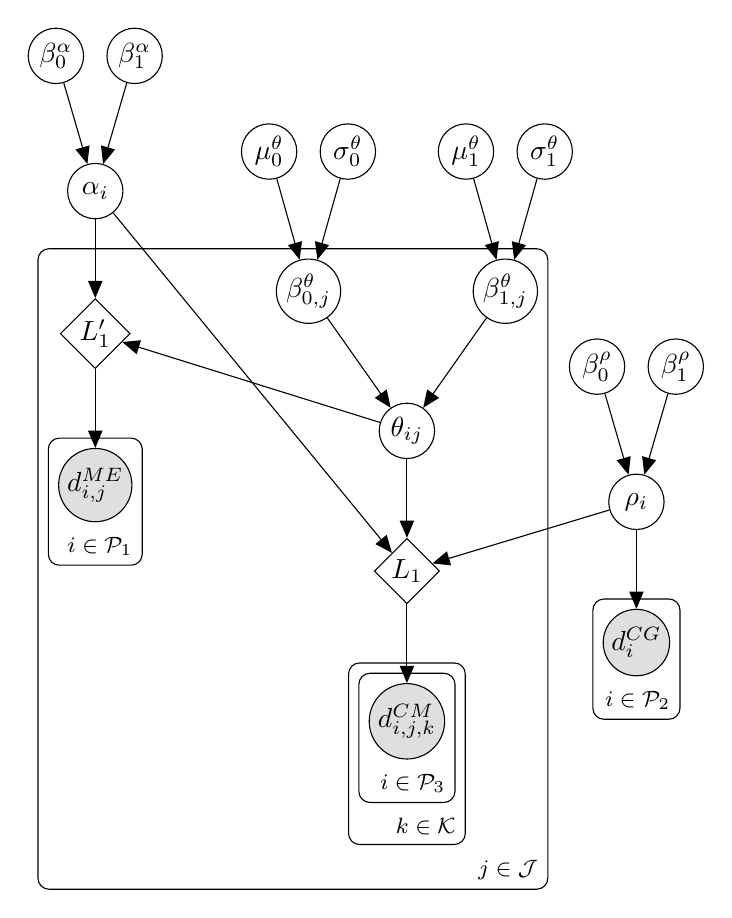
\begin{tikzpicture}
	%% RSA nodes and data
	\node[obs](data_comb){$d^{CM}_{i, j, k}$};
	\node[obs, left=3 of data_comb, yshift=3cm](data_me){$d^{ME}_{i, j}$};
	\node[obs, right=2 of data_comb, yshift=1cm](data_cg){$d^{CG}_{i}$};
	
	\node[det, above=of data_me](L1_me){$L'_1$};
	\node[det, above=of data_comb](L1_comb){$L_1$};
	
	\edge{L1_me}{data_me};
	\edge{L1_comb}{data_comb};
	
	% COMMON GROUND
	\node[latent, above=of data_cg](rho){$\rho_i$};
	\node[latent, above=of rho, xshift=-0.5cm](beta_rho_int){$\beta^{\rho}_0$};
	\node[latent, above=of rho, xshift=0.5cm](beta_rho_slope){$\beta^{\rho}_1$};
	
	\edge{rho}{data_cg};
	\edge{beta_rho_int}{rho};
	\edge{beta_rho_slope}{rho};
	\edge{rho}{L1_comb};
	
	%% SPEAKER INFORMATIVITY
	
	\node[latent, above=of L1_me](alpha){$\alpha_i$};
	\node[latent, above=of alpha, xshift=-0.5cm](beta_alpha_int){$\beta^{\alpha}_0$};
	\node[latent, above=of alpha, xshift=0.5cm](beta_alpha_slope){$\beta^{\alpha}_1$};

	\edge{alpha}{L1_me};
	\edge{beta_alpha_int}{alpha};
	\edge{beta_alpha_slope}{alpha};
	\edge{alpha}{L1_comb};
	
	%% SEMANTIC KNOWLEDGE model

	\node[latent, above=of L1_comb](theta){$\theta_{ij}$};
	\node[latent, above=of theta, xshift=-1.25cm](beta_theta_int){$\beta^{\theta}_{0, j}$};
	\node[latent, above=of theta, xshift=1.25cm](beta_theta_slope){$\beta^{\theta}_{1, j}$};
	
	\node[latent, above=of beta_theta_int, xshift=-0.5cm](mu_theta_int){$\mu^{\theta}_{0}$};
	\node[latent, above=of beta_theta_int, xshift=0.5cm](sigma_theta_int){$\sigma^{\theta}_{0}$};
	
	\node[latent, above=of beta_theta_slope, xshift=-0.5cm](mu_theta_slope){$\mu^{\theta}_{1}$};
	\node[latent, above=of beta_theta_slope, xshift=0.5cm](sigma_theta_slope){$\sigma^{\theta}_{1}$};
	
	\edge{theta}{L1_me};
	\edge{theta}{L1_comb};
	\edge{beta_theta_int}{theta};
	\edge{beta_theta_slope}{theta};
	\edge{mu_theta_int}{beta_theta_int};
	\edge{sigma_theta_int}{beta_theta_int};
	\edge{mu_theta_slope}{beta_theta_slope};
	\edge{sigma_theta_slope}{beta_theta_slope};
	
	\plate{plate_data_me}{
		(data_me)
	}{$i \in \mathcal{P}_{1}$}
	
	\plate{plate_data_comb}{
		(data_comb)
	}{$i \in \mathcal{P}_{3}$}

	\plate{plate_data_cg}{
		(data_cg)
	}{$i \in \mathcal{P}_{2}$}
	
	\plate{plate_condition}{(plate_data_comb)}{$k \in \mathcal{K}$};
	
	\plate{plate_items}{
		(plate_data_me)
		(plate_data_comb)
		(plate_condition)
		(L1_me)
		(L1_comb)
		(theta)
		(beta_theta_int)
		(beta_theta_slope)
	}{$j \in \mathcal{J}$}
			
\end{tikzpicture}

    \end{tabular}
  \end{center}
  \caption{ Put a caption here.}
  \label{fig:bayesnet}
\end{figure}




\end{document}

